
\chapter{L'estimation}

Pour effectuer la planification sur Microsoft Project, une estimation préalable de la durée des tâches est nécessaire. 

\section{Estimation de la partie analyse}

L’estimation des charges de la partie hors développement se résume en deux grands points : le temps passé en réunion ainsi que le temps passé pour la rédaction des rapports et à la préparation des soutenances. Cette partie n’a pas été la plus complexe à estimer car nous avons pu nous baser sur les temps passés lors des trois premiers mois du projet où nous nous sommes concentrés sur la compréhension du cahier des charges et la planification du projet.

\paragraph{}

Dans un premier temps, des créneaux horaires nous sont accordés dans l’emploi du temps pour les réunions. Le temps de réunion correspond au temps accordé dans ces créneaux, à savoir 3 heures par semaine. Dans un  second temps, nous avons calculé le temps nécessaire à la réalisation des prochains rapports.  Pour ce faire nous avions besoin de plusieurs chiffres :

\begin{itemize}
\item le nombre moyen d’heures passées par personnes pour la réalisation d’un rapport. Ce chiffre est basé sur le temps que nous avons passé pour l’écriture des premiers rapports, soit environ 1h30 de travail pour rédiger la première version d’un rapport ;
\item le nombre de personnes affectées à la rédaction d’un rapport. Nous avons choisi de mobiliser l’intégralité du groupe pour l‘écriture de chaque rapport, ce choix a été fait lors du travail sur le diagramme de Gantt, il sera expliqué dans la partie suivante. Pour les rapports déjà rendus, il y avait donc 8 personnes à travailler dessus.
\end{itemize}

\paragraph{}

En multipliant ces chiffres, nous avons obtenu la charge des rapports, chacun représente donc une dizaine d’heures de travail en moyenne. Ce calcul a été possible car nous avons réparti de façon homogène entre les membres du groupe la charge de travail pour la réalisation des rapports.

\section{Estimation de la partie développement}

Cette partie a été plus compliquée à estimer car nous avions peu de repères. Pour nous rapprocher au maximum d’une estimation fiable, nous avons estimé le temps de développement de chaque partie en considérant les points suivants : 

\begin{itemize}
\item connaissance des technologies utilisées (donc temps d’apprentissage nécessaire estimé) ;
\item temps estimé de conception ;
\item temps estimé de développement (en incluant les tests et la documentation) .
\end{itemize}

\paragraph{}

La somme de ces estimations nous a donné l’estimation du temps de développement pour chaque bloc, en ajoutant une marge de sécurité.

\subsection{Estimation du temps d'apprentissage}

Les différentes technologies qui seront utilisées ont été définies dans le rapport de spécification. Nous savons donc déjà quelles technologies devront être apprises avant de commencer le développement. Le temps d’apprentissage a été défini grossièrement en nous basant sur notre expérience d’auto-formation sur des langages ou d’autres types de technologie.

\subsection{Estimation du temps de conception}

La conception ayant majoritairement été réalisée précédemment, cette partie est presque inexistante. Cependant, il est possible que la conception réalisée soit éloignée des réalités techniques. Nous avons donc inclus dedans un temps de remodélisation si nous nous rendons compte à un moment que notre première modélisation n’était pas applicable.

\subsection{Estimation du temps de développement}

Cette partie de l’estimation est la plus compliquée à estimer. En effet, il n’est pas possible de prévoir les problèmes que nous allons rencontrer. C’est pourquoi, nous nous sommes basés sur le temps de développement d’autres projets que nous avons réalisés comptant l’écriture du code, la documentation ainsi que les tests. Afin d’essayer d’obtenir une approximation plus proche de la réalité, nous avons divisé en plus petites parties les objectifs de chacun. Ainsi, alors qu’un grand projet peut paraître vague à estimer, raisonner sur des petites parties concrètes nous permet cette granularité.

\subsection{Résumé}

Nous avons donc décomposé chaque tâche en sous-parties. Tout d’abord une marge de 25\% est définie en cas de sous-estimation du temps de travail. Ensuite, le travail à faire est décomposé en deux grande parties auxquelles un temps égal est accordé : la conception de la solution en elle-même (contenant les phases d’apprentissage et de conception, ainsi que le développement) et la correction de la solution (comprenant les tests, l’intégration et la documentation). Concernant la première partie, 12.5\% du temps correspond à l’analyse du travail à faire, à la recherche d’une solution efficace pour répondre au problème posé. Le développement en temps que tel, l’implémentation de la réponse, représente 25\% du temps. Concernant la seconde partie, 20\% du temps est accordé à la création et à l’exécution de tests afin de vérifier le bon fonctionnement de la solution. Enfin, respectivement 12.5\% et 5\% sont dédiés à l’intégration au sein du projet et à la documentation. Ces pourcentages sont bien évidemment approximatifs et varient en fonction de la tâche.

\newpage

\begin{mdframed}[frametitle={Figure 1 : Diagramme de répartition du travail par tâche}, innerbottommargin=10]
\begin{center}
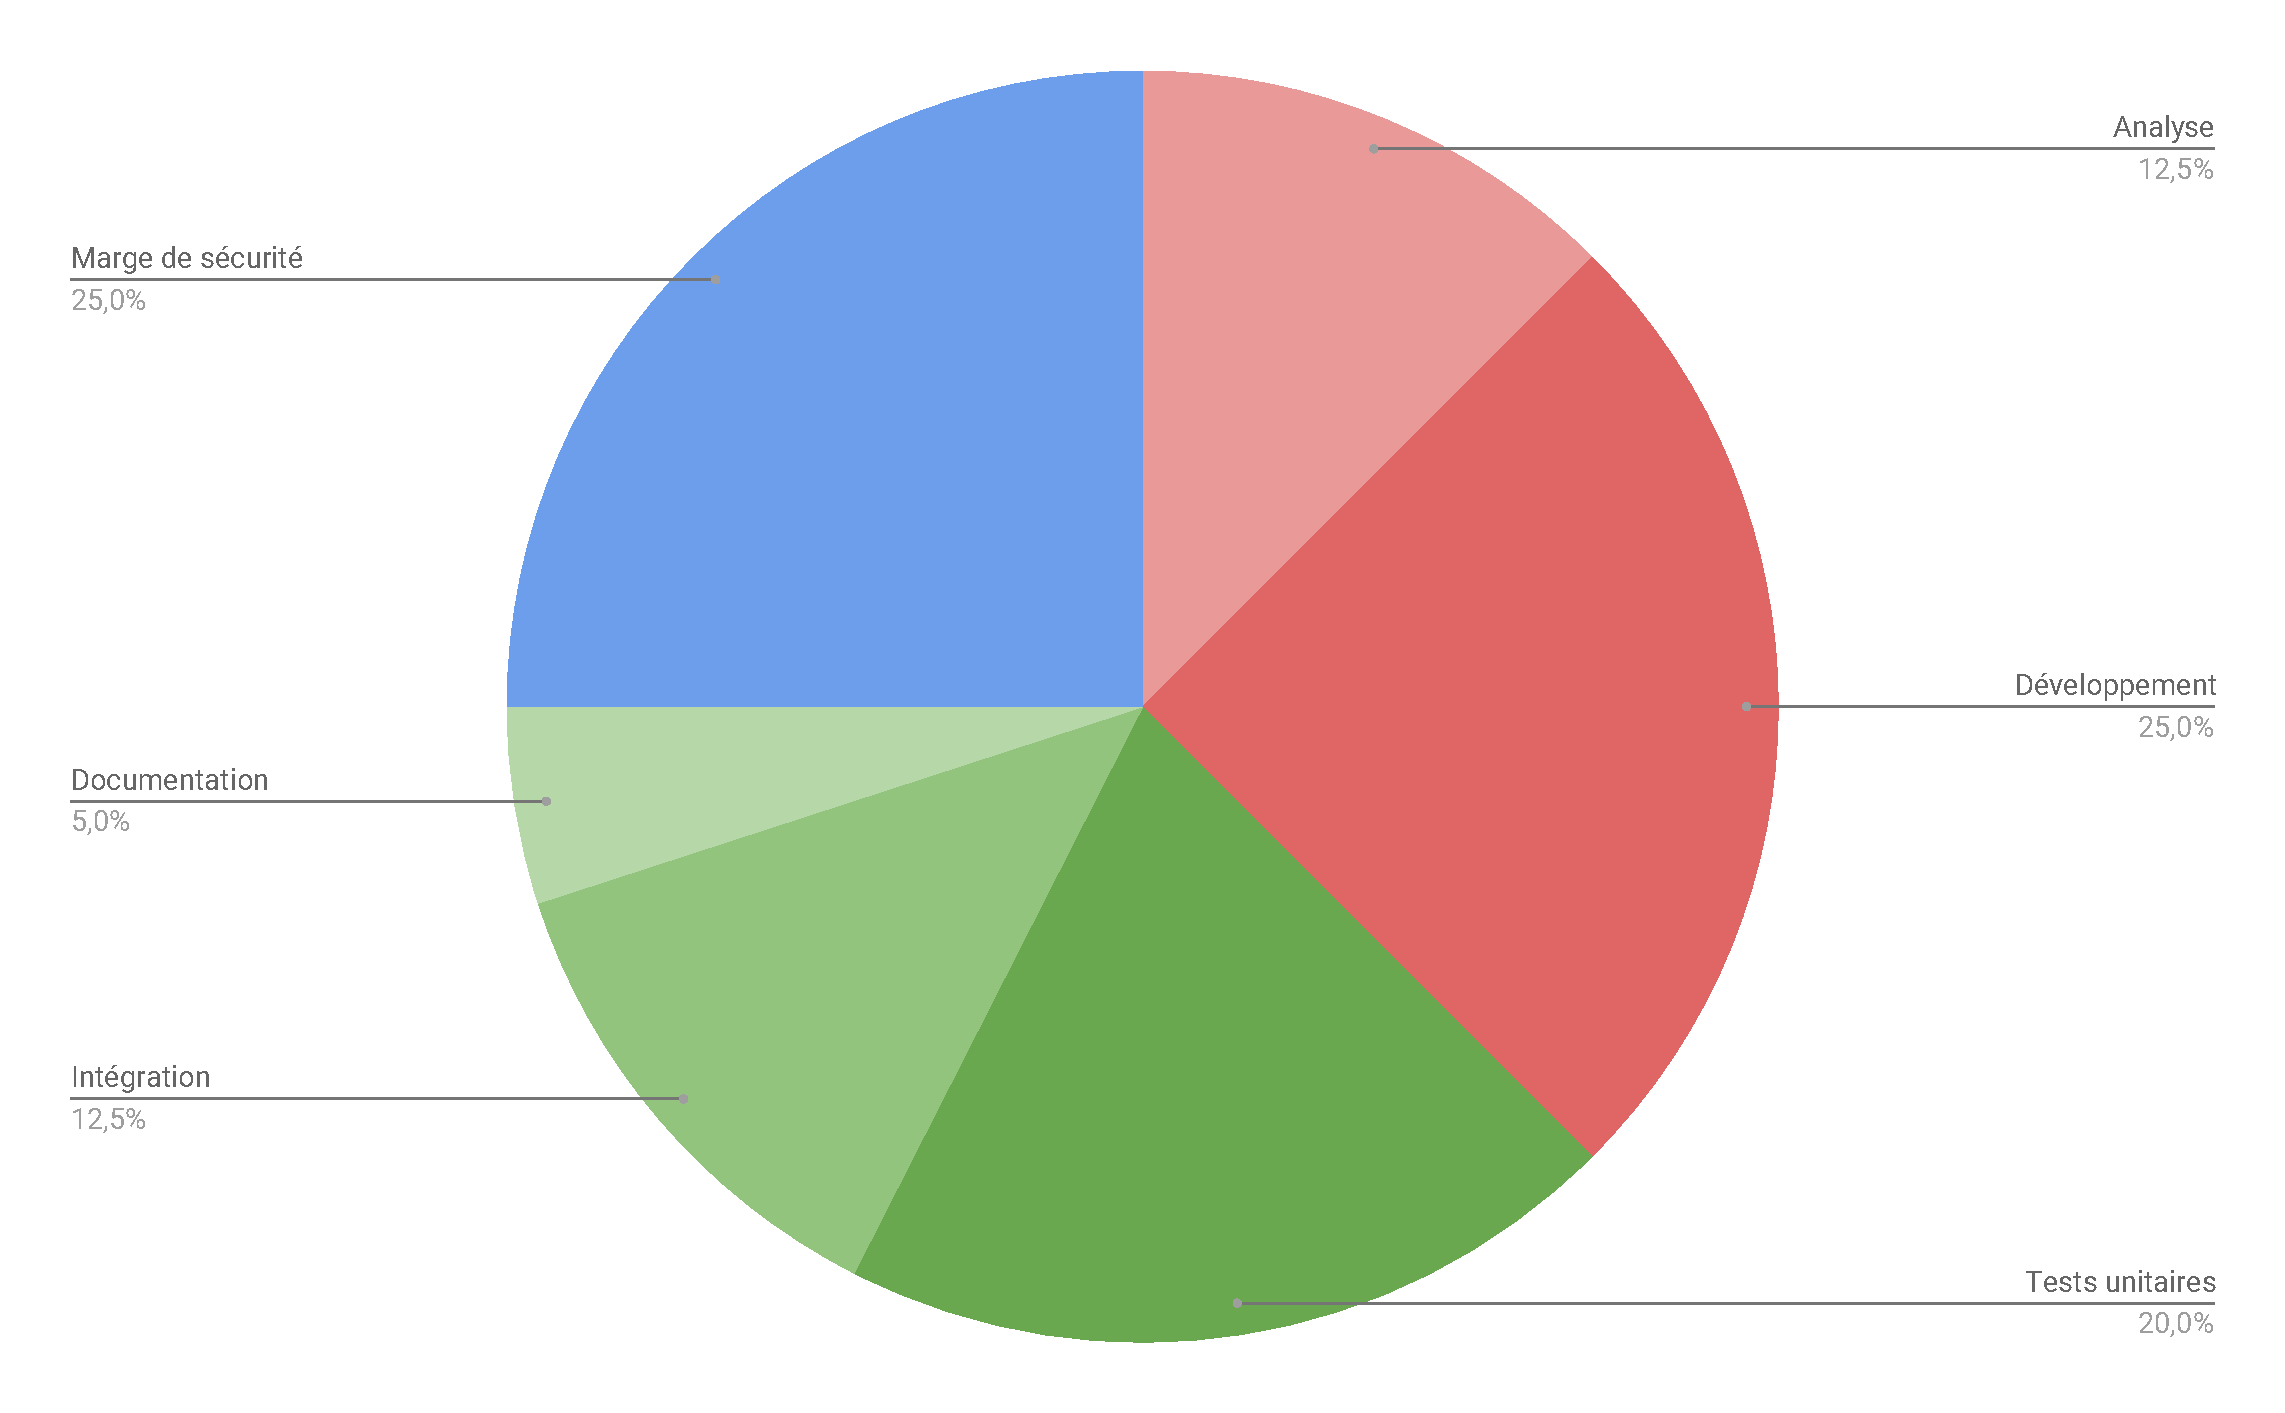
\includegraphics[scale=0.44]{repartition_travail_taches.pdf}
\end{center}
\end{mdframed}

\paragraph{}

\paragraph{}

Par exemple, 10 heures de travail ont été estimées pour la tâche Conversion des données au format d’entrée du reconnaisseur (spécification IR\_CV). Cette tâche consiste en la conversion des données extraites de la base en un format compatible avec le reconnaisseur. 1 heure est accordée à l’apprentissage, 1 heure à la conception. Tous les éléments à créer ayant déjà été vus en cours (patrons de conception MOO) ou au cours du projet (les formats d’entrée ont été étudiés au cours de la pré-étude). 2 heures sont accordées au développement (le temps standard d’un TP). Une quantité égale de temps est prévue pour les tests, soient 4 heures, cette tâche étant un préalable à de nombreuses tâches suivantes du projet. Enfin 2 heures sont laissée comme marge de sécurité.


